\chapter{Implementation Details}
In this chapter, we will describe the details on how we implemented the application. We will start explaining the architecture from a high-level perspective with each component being a blackbox. Later sections of this chapter will then further describe the internals of each component of our system.
\section{Component Overview}
From a high-level perspective, our application consists of three components which themselves may consist of multiple sub components:
\begin{itemize}
	\item Web application
	\item Backend
	\begin{itemize}
		\item REST Service
		\item Datasync Service
		\item VoteSimulation
	\end{itemize}
	\item CHVote crypto-library
\end{itemize}
%TODO: Component diagram %

\subsection{Technologies and Frameworks}
Since the CHVote crypto-library has been already implemented in python during project II, python was also the obvious choice for the backend. \textbf{Python} offers a wide variety of frameworks for building webservices. Since we planed on building a singlepage-application for the client, we chose the lightweight micro-framework flask for building a restful webservice. \textbf{Flask} also offers support for websockets and the popular websocket framework socket.io, which we used also in our frontend. \textbf{Socket.io} simplifies the usage of websockets and offers fallback technologies such as longpolling in case websocket is not supported by the browser or the webserver. For persisting the state of an election between the stateless API/webservice calls, we use mongoDB to store the states of all parties of an election.

For our frontend (web application) we evaluated several singlepage application (SPA) frameworks. \textbf{VueJS} is a new, modern and lightweight SPA framework that in contrast to Angular has a much flatter learning curve but still offered all the functionality that we needed. The VueJS addon Vuex enabled us to establish a datastore pattern in our frontend, which makes it possible to have a copy of the backend datastore in our web application which is synchronized in real-time through socket.io.

More about how these technologies and frameworks are used and the communication between these components is described in more details in the following sections.

\section{Architecture}
The core of our application is the VoteSimulation component in our backend which implements the evoting protocol by utilizing all algorithms of the CHVote crypto-library according to the CHVote specification. The VoteSimulation component internally holds the state of a whole CHVote election and exposes functions to manipulate this state at a granularity required by our web application to implement all usecases. For example: The VotingSimulation contains a list of ballots and exposes functions to cast a new ballot, which will generate a new ballot according to the protocol, by calling the CHVote crypto-library, and adds the ballot to the ballotlist.

On top of the VoteSimulation we have implemented a REST service that acts a facade to the VoteSimulation component and makes it's functionality available as an API for our webclient. The REST service also has to initialize the VoteSimulation by loading and persisting it's state from and to the database between each API call.

Since it's a requirement that all clients of a particular election must be notified of mutations of the state, we have implemented a data sync service which allows to push the state or parts of the state of the VoteSimulation to the webclients by using the websocket protocol. This service is utilized by the REST service after every API call that could have potentially manipulated the state.

To establish a proper separation of concerns, the state of the VoteSimulation is always sent to the client via the data sync service. The REST service only returns success or error codes or information that is required in response to some particular API call, and never state objects. On the other hand, the data sync service does never manipulate the state of the VoteSimulation and is solely responsible for sending data to the client.

\begin{figure}[h!]
\begin{center}
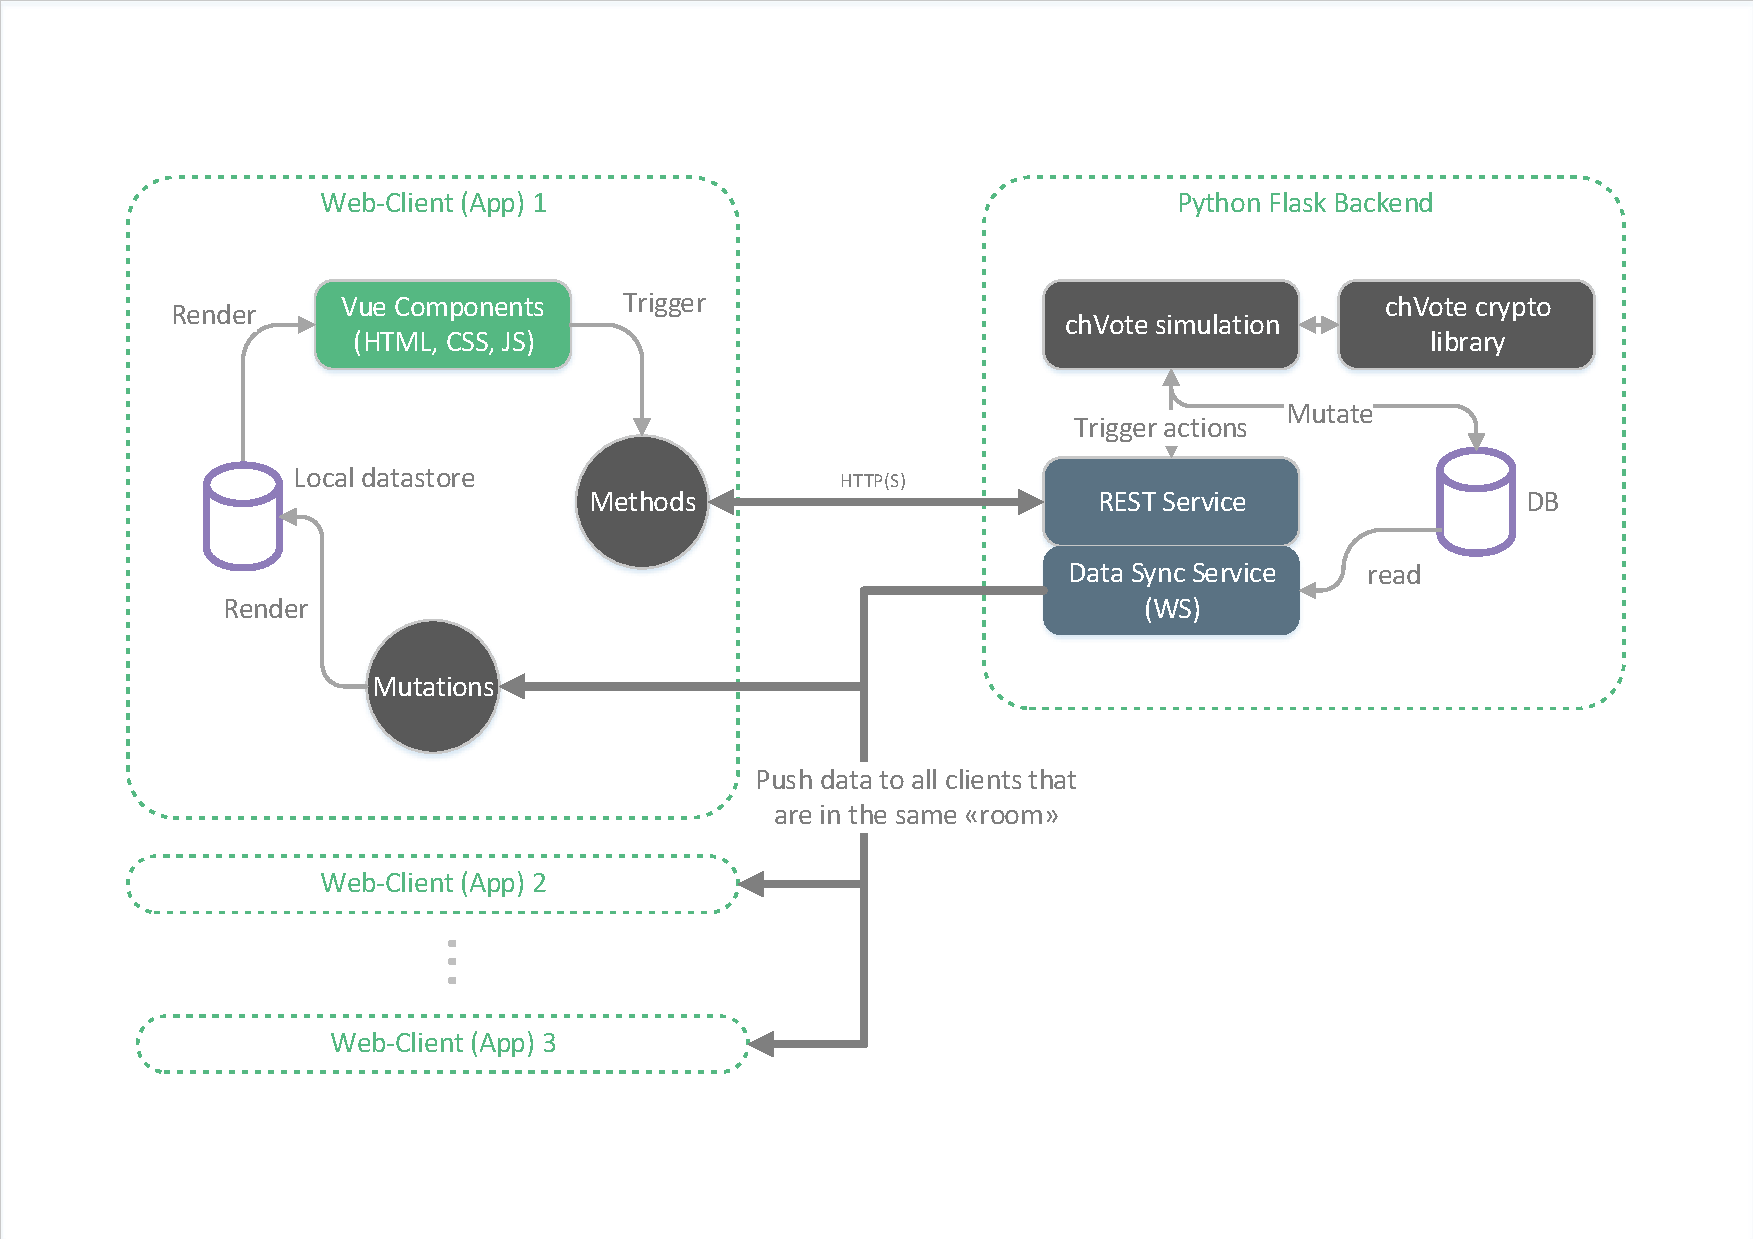
\includegraphics[scale=0.62]{assets/architecture.pdf}
\caption{Architecture}
\end{center}
\end{figure}

From the clients point of view, the webclient contains a copy of the whole VoteSimulation state in a local datastore. This store is initially populated when the web application is initialized with an election. Whenever the state of the VoteSimulation changes, the data sync service is is called to push the new data to the web application. A local mutation handler is called inside the web application which writes the new data into the local datastore.

Since the components that the webpages of the web application are built of, are directly bound to the local datastore, all mutations automatically reflected to the user. From those pages, the REST API can be called to trigger some CHVote specific action on the backend. The resulting state change is again being pushed to all clients while the responsible client that performed the HTTPS request will additionally receive a success code, or an error message in case of an error.

\section{Backend}
The backend mainly consists of the VoteSimulation which implements the CHVote protocol by using the CHVote crypto-library. 
\subsection{VoteSimulation}
We have divided the state of a CHVote election into the following classes:
\begin{itemize}
	\item \textbf{BulletinBoardState}: Holds all data that is publicly available on the bulletin board (the number of candidates, the tallied result)
	\item \textbf{ElectionAuthorityState}: Holds all data that an election authority knows (e.g. the list of ballots, the secret key of an election authority)
	\item \textbf{VoterState}: Since there is no distinction made between a voter and a voting client in our application, the VoterState contains the data of both the voter (e.g. the voting card) and the data typically known to the voting client (e.g. the points returned by the oblivious transfer)
	\item \textbf{PrintingAuthorityState}: Holds the data known to the printing authority (e.g. the list of all voters private credentials and the voting cards)
	\item \textbf{ElectionAdministratorState}: Holds all data known to the election administrator 
\end{itemize}

Since our application must handle multiple elections in parallel, the state cannot be kept in RAM, but needs to be persisted between every single request. For this reason we evaluated different database systems and concepts. We decided not to use a relational database system that requires us to define a database schema as we want our state objects to be the only place where the schema is defined. This makes it easier to apply changes to the protocol in future. 

For our purpose, mongoDB seemed like a good choice. Since we do not need the ability to access and filter our data with arbitrary queries, but only need to be able to save and load a state object of a particular election, we simply store the whole state as a binary string in a mongoDB collection. The only additional attribute that is saved to the database alongside with the serialized state is the electionId which denotes which election a particular state belongs to. 

An election contains multiple VoterStates and ElectionAuthorityStates. Therefore, these two states additionally require an electionAuthorityId and a voterId.

% TODO : Grafik der MongoDB collections / Struktur %

The only common functionality between every state object, is the ability to serialize the object to a JSON string. For this reason we had to write a custom transformer which tells the JSON parser how to serialize datatypes such as mpz, bytearrays and custom classes. Luckily, python offers a way to easily serialize any custom object. By calling \mintinline{python}/object.__dict__/ we can convert an object into a dictionary, as long as transformer is able to serialize all properties of the object.

\subsection{Actor/Party-classes}
We described how the state classes are used to divide the data of the VoteSimulation into smaller units. Similarly, the functionality of the VoteSimulation class is separated into classes, one for every actor in the protocol.

% TODO: Diagram %

The common functionality, namely, a function for loading the corresponding state from the database and one for persisting the state to the database, are contained in an abstract base class.

\subsection{REST Service}
\subsection{Data-Sync Service}

The following sequence diagram shows how the vote casting use case is implemented within the backend.
\begin{figure}[h!]
\begin{center}
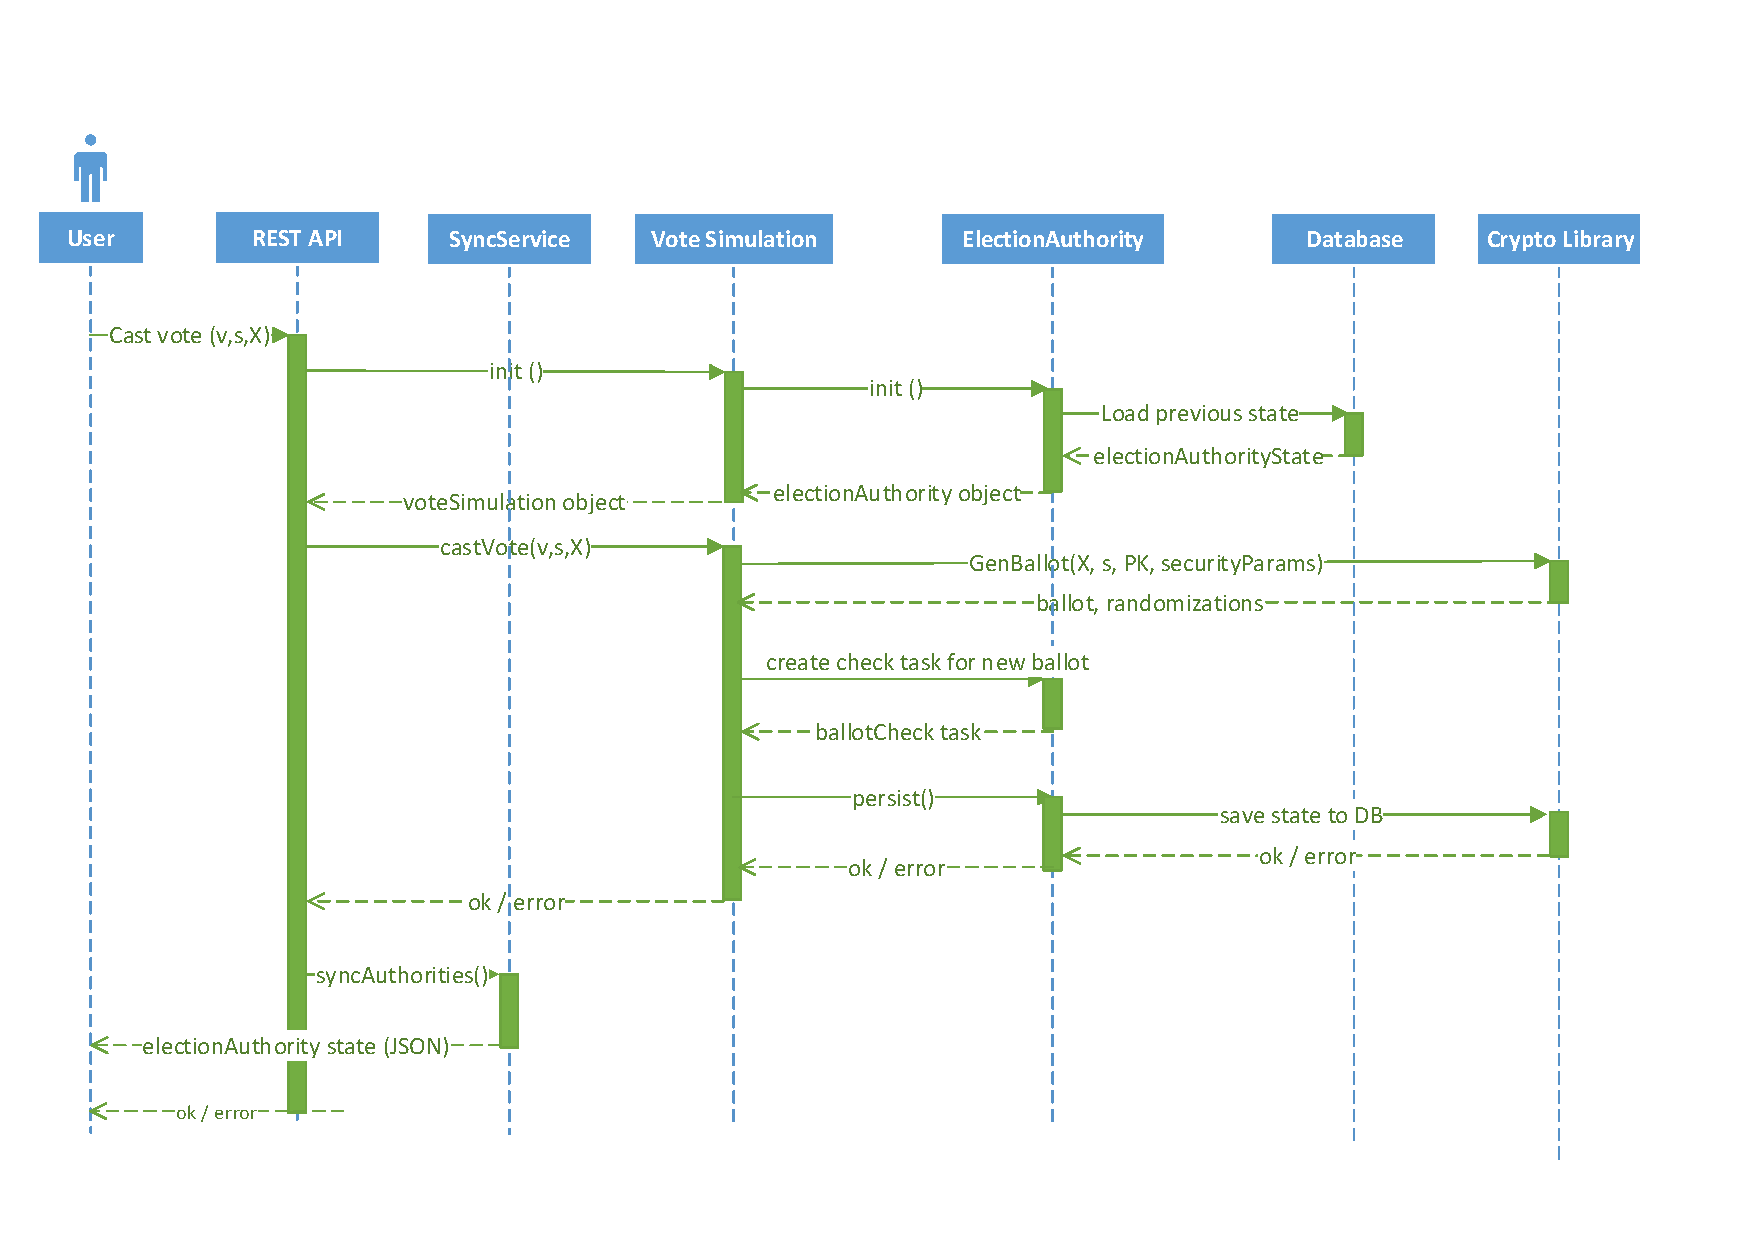
\includegraphics[scale=0.65]{assets/votecastingDiagram.pdf}\\
\caption{Vote casting sequence diagram}
\end{center}
\end{figure}

\section{Crypto-library}
\section{Language choice}
As both team members are working in different fields of employment and are experienced in different programming languages, there wasn't an obvious choice as in what programming language we would implement this project. Also, as Java has already been used by the team in Geneva, Java was out of question. Different programming languages have been taken into consideration and in the end Python seemed like a rather suitable language due to the following reasons:

\begin{itemize}
	\item simple syntax and commonly known language features
	\item mature language and standard libraries
	\item python's syntax enables programs to be written in a compact and readable style
	\item native support for large integers (\textit{BigInts}) and bindings for the GMP\footnote{GMP is a free library for arbitrary precision arithmetic, operating on signed integers, rational numbers, and floating-point numbers, see \url{https://gmplib.org/}.} library
	\item supports a lot of platforms
	\item many popular web development frameworks are implementated in Python
\end{itemize}

Throughout the project not all of the reason above turned out to be true or ideal. The drawbacks that we have experienced during the implementation of this project will be discussed at the end of this document.

\subsection{Project structure}
We decided to put every algorithm of the specification in its own file together with related unit tests. The files are structured according to the actors of the protocol, for example:

\begin{itemize}
	\item \textbf{Common}: contains common cryptopgraphic algorithms and the security parameters used by multiple algorithms
	\item \textbf{ElectionAuthority}: contains all the algorithms used by the election authority
	\item \textbf{PrintingAuthority}: contains all the algorithms used by the printing authority
	\item \textbf{VotingClient}: contains all the algorithms used by the voting client
	\item \textbf{ElectionAdministration}: contains all the algorithms used by the election administrator
	\item \textbf{Utils}: contains helper classes and miscellaneous utility functions
\end{itemize}

\subsection{Public parameters}
There exist two types of public parameters:

The \textbf{security relevant parameters}, e.g:

\begin{itemize}
	\item The order of the prime groups: $p$, $\prime{p}$, $\hat{p}$
	\item The length of the voting, confirmation, return and finalization codes
	\item The number of authorities: $s$
\end{itemize}

and \textbf{public election parameters}, e.g.:

\begin{itemize}
	\item The size of the electorate: $N_E$
	\item The number of candidates: $n$
	\item The list of candidate descriptions: $c$
\end{itemize}

The security parameters are typically used within the algorithms and remain unchanged for a longer time period, whereas the public election parameters are only used by the protocol implementations and change with every election.

The object \texttt{SecurityParams} holds all security relevant parameters and is injected as an additional function argument to all algorithms. Several different \texttt{SecurityParams} objects are created initially, which contain all the parameters according to the recommendations in the CHVote specification document ("level 0" for testing purposes and "level 1" through "level 3" for actual use of the protocol). This approach allows us to use different levels of security during development of the algorithms and protocols. For simple unit testing we used "level 0" in order to inject the security parameters recommended for testing puposes. For actual test runs of the project the security parameters from "level 2" were used.

The public election parameters on the other hand are directly passed to the algorithms by the calling party. If an algorithm needs to know certain election parameters (like the size of the electorate $N_E$), these values are typically derived from vectors that they have access to, so they do not require specific knowledge of these parameters.

\subsection{Coding style}
The following source code sample shows a typical implemation of an algorithm (in this exmaple, algorithm 7.18 according to the CHVote specification).

\begin{minted}[linenos,tabsize=2,breaklines]{python}
import unittest
import os, sys
from gmpy2 import mpz
import gmpy2

sys.path.append(os.path.dirname(os.path.dirname(os.path.abspath(__file__))))

from Utils.Utils                    import AssertMpz, AssertList, AssertClass, AssertString
from Crypto.SecurityParams          import SecurityParams, secparams_l0
from Utils.ToInteger                import ToInteger
from VotingClient.GetSelectedPrimes import GetSelectedPrimes
from VotingClient.GenQuery          import GenQuery
from VotingClient.GenBallotProof    import GenBallotProof
from UnitTestParams                 import unittestparams
from Types                          import Ballot
from Utils.StringToInteger          import StringToInteger

def GenBallot(X_bold, s, pk, secparams):
    """
    Algorithm 7.18: Generates a ballot based on the selection s and the voting code X. The
    ballot includes an OT query a and a proof pi. The algorithm also returns the random
    values used to generate the OT query. These random values are required in Alg. 7.27
    to derive the transferred messages from the OT response, which itself is generated by Alg. 7.25.

    Args:
        X_bold (str):                       Voting Code X ∈ A_X^l_X
        s (list of int):                    Selection s = (s_1, ... , s_k), 1 <= s_1 < ... < s_k
        pk (mpz):                           ElGamal key pk ∈ G_p \ {1}
        secparams (SecurityParams):         Collection of public security parameters

    Returns:
        tuple:                              alpha = (r, Ballot) = (r, (x_hat, a, b, pi))
    """

    AssertMpz(pk)
    AssertList(s)
    AssertClass(secparams, SecurityParams)

    x = mpz(StringToInteger(X_bold, secparams.A_X))
    x_hat = gmpy2.powmod(secparams.g_hat, x, secparams.p_hat)

    q_bold = GetSelectedPrimes(s, secparams)                    # q = (q_1, ... , q_k)
    m = mpz(1)

    for i in range(len(q_bold)):
        m = m * q_bold[i]

    if m >= secparams.p:
        return None

    (a_bold, r_bold) = GenQuery(q_bold, pk, secparams)
    a = mpz(1)
    r = mpz(0)

    for i in range(len(a_bold)):
        a = (a * a_bold[i]) % secparams.p
        r = (r + r_bold[i]) % secparams.q

    b = gmpy2.powmod(secparams.g,r, secparams.p)
    pi = GenBallotProof(x,m,r,x_hat,a,b,pk, secparams)
    alpha = Ballot(x_hat,a_bold,b,pi)

    return (alpha, r_bold)

class GenBallotTest(unittest.TestCase):
    def testGenBallot(self):
        selection = [1,4]       # select candidates with indices 1,4
        (ballot, r) = GenBallot(unittestparams.X, selection, unittestparams.pk, secparams_l0)
        print(ballot)
        print(r)

if __name__ == '__main__':
    unittest.main()
\end{minted}

All algorithms contain a short description, which was taken as-is from the specification document, as well as a comment (Google-style documentation string), which can be used to automatically generate code documentation. The algorithm itself is implemented as close to the specification as possible, using the same variable names and (as far as the language supports it) similar control structures:

\begin{itemize}
	\item The suffix \texttt{\_bold} for emphasized (bold) variables, e.g. \texttt{p\_bold} for \textbf{p}
	\item The suffix \texttt{\_hat} for variables with a hat, e.g. \texttt{a\_hat} for $\hat{a}$
	\item The suffix \texttt{\_prime} for variables with a prime, e.g. \texttt{a\_prime} for $a'$
	\item etc.
\end{itemize}

Each file also contains unit test relevant to the specific algorithm (if unit testing was considered useful for the particular algorithm).

The following example shows the similarities between the algorithm pseudo code and the actual implmentation in Python:

\begin{multicols}{2}
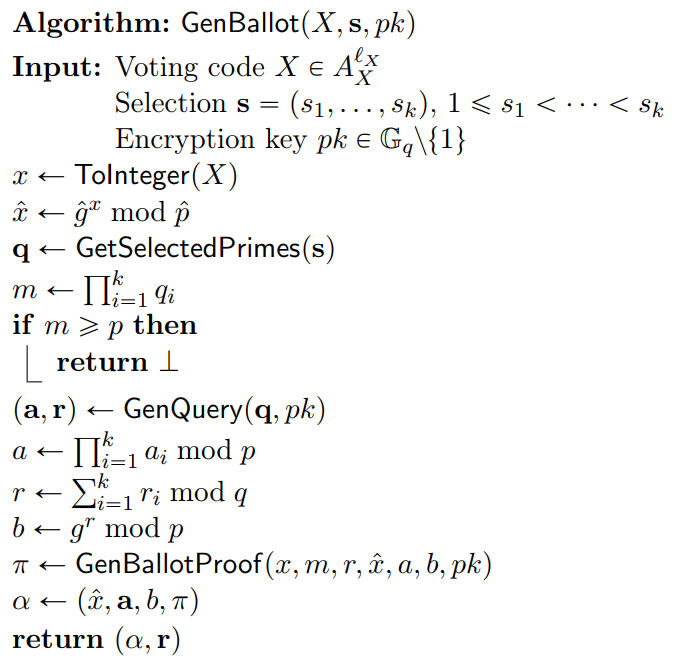
\includegraphics[width=0.46\textwidth]{assets/genballot.png}
\columnbreak
\begin{minted}[fontsize=\scriptsize]{python}
x = mpz(StringToInteger(X_bold, secparams.A_X))
x_hat = gmpy2.powmod(secparams.g_hat, x, secparams.p_hat)
q_bold = GetSelectedPrimes(s, secparams)

m = mpz(1)
for i in range(len(q_bold)):
    m = m * q_bold[i]

if m >= secparams.p:
    return None

(a_bold, r_bold) = GenQuery(q_bold, pk, secparams)
a = mpz(1)
r = mpz(0)

for i in range(len(a_bold)):
    a = (a * a_bold[i]) % secparams.p
    r = (r + r_bold[i]) % secparams.q

b = gmpy2.powmod(secparams.g,r, secparams.p)
pi = GenBallotProof(x,m,r,x_hat,a,b,pk, secparams)
alpha = Ballot(x_hat,a_bold,b,pi)

return (alpha, r_bold)
\end{minted}
\end{multicols}

\subsection{Return types}
In most cases, when an algorithm returns more than a scalar datatype, tuples are used. Tuples allow to return multiple values from a function:

\begin{minted}[linenos,tabsize=2,breaklines]{python}
def foo():
   return (1, 2)

def main():
   a, b = foo()
\end{minted}

This way a lot of the source code looked very similar to the pseudo code in the CHVote specification. For more complex data types or return values that are used more often, named tuples were used. The data type "namedtuple" is like a lightweight class and allows access to named properties.

\begin{minted}[linenos,tabsize=2,breaklines]{python}
Ballot = namedtuple("Ballot", "x_hat, a_bold, b, pi")

def main():
   Ballot b = getBallot()
   x_hat = b.x_hat
\end{minted}

By following this approach we can avoid having lots of container classes only used to pass data structures between the algorithms.

\section{Frontend}
Our frontend is a singlepage application built with Javascript, VueJS, HTML5 and CSS3. We tried to follow the design patterns and best practices proposed by the VueJS framework wherever possible.

Every site of our applications consists of at least one VueJS component which is activated when the user visits the corresponding route in the URL.
\subsection{Datastore}
The web application's datastore is divided into multiple modules, one datastore module for each corresponding state of the backend.

TODO: Grafik die zeigt, wie VueX Datastores mit Backend States zusammenhängen
 
\subsection{Websocket room concept}
TODO: Konzept mit den Rooms / Election IDs beschreiben

\subsection{Development Environment}
TODO: Webpack, ESlint etc. beschreiben